\documentclass[11pt, oneside]{article} 
\usepackage{geometry}
\geometry{letterpaper} 
\usepackage{graphicx}
	
\usepackage{amssymb}
\usepackage{amsmath}
\usepackage{parskip}
\usepackage{color}
\usepackage{hyperref}

\graphicspath{{/Users/telliott/Dropbox/Github-Math/figures/}}

\title{Congruence of triangles}
\date{}

\begin{document}
\maketitle
\Large

%[my-super-duper-separator]

\subsection*{side-side-side, SSS}

Congruence is a fancy word for equal, or "the same".

Here is a fundamental theorem about congruency for triangles:

$\bullet$  Two triangles are \emph{congruent} if and only if they have the same three side lengths. 

This test is often abbreviated SSS (side-side-side). 

By definition, a triangle and its mirror image are congruent.  The three triangles shown below are all congruent, even though two are flipped (they are mirror images).

\begin{center} \includegraphics [scale=0.4] {congruent.png} \end{center}

Having three sides equal means that the shape is the same.  The three angles are also equal --- and the shapes are superimposable, with the understanding that we allow one triangle to be flipped over.

You may wonder why this is so.  Draw one side of a triangle, and from its endpoints draw circles with radii the length of the other two sides.

\begin{center} \includegraphics [scale=0.4] {congruent4.png} \end{center}

The two radii map out all the points that are the same distance from the centers.  Thus they include all the possibilities for three given side lengths.

We see that the radii cross at two and only two different points, which have mirror image symmetry above and below the original base (black line).  Thus, three given side lengths can only be drawn together to give two resulting triangles, and these two shapes are mirror images.

\subsection*{other tests}

In addition to SSS, there are three other conditions that always lead to congruence of two triangles when they are satisfied, namely

$\circ$  SAS (side-angle-side)

$\circ$  ASA (angle-side-angle)

$\circ$  AAS (angle-angle-side)

When any one of these is true then SSS is also true. 

Note:  when we say SAS, we mean that the two sides are adjacent and the angle we know lies between them.  Similarly, ASA means that we have a side of a triangle and the two angles at either end of that side are the angles in question.

Sometimes triangles are \emph{similar}, but not congruent.

Similarity means that the three angles are the same but the triangles are of different overall sizes.  

We might say that they are the same but \emph{scaled} differently.  

We call this criterion AAA (angle-angle-angle).  For similar triangles, the three corresponding pairs of sides are in the same proportions, but re-scaled by a constant of proportion.

\begin{center} \includegraphics [scale=0.4] {similar2.png} \end{center}

Because of the triangle sum theorem (\hyperref[sec:triangle_sum_theorem]{\textbf{ref}}), if any two angles of a pair of triangles are known to be equal, then the third one must be equal as well.

\subsection*{constructions}

A good way to think about the congruence conditions is to imagine trying to construct a triangle from the given information, and ask whether it is uniquely determined.  

We already did SSS above.  SAS is also easy.

\begin{center} \includegraphics [scale=0.4] {SAS2.png} \end{center}

Two sides and the angle between them are given.  So draw that part of the triangle.  Notice that the second and third vertices are also determined, they are just at the ends of the two sides we're given.  All that remains is to draw the line segment joining them.

The next one is ASA.  Since we know two angles, we know the third.  Here is a diagram of the situation:

\begin{center} \includegraphics [scale=0.4] {ASA1.png} \end{center}
 
Draw the known side, then using the known angles, start two other sides from the ends of that side.  They must cross at a unique point.  This follows from the parallel postulate and the fact that the sum of two angles in a triangle must be less than two right angles.

But... actually, if we start the two lines from opposite ends of the horizontal

\begin{center} \includegraphics [scale=0.4] {ASA4.png} \end{center}

there is another solution, the mirror image.  These two triangles are congruent to the one above.
 
If we know two angles we also know the third, by the triangle sum theorem.  For this reason, ASA and AAS mean that we have exactly the same information, because we know all three angles and we know one side.

Crucially, we know \emph{which} two angles flank the known side.  Equivalently, it is enough to know which angle is opposite to the known side.
 
\subsection*{SAS, ASA, AAS but not SSA}

We need some way of marking sides and angles to show they are equal.  Here is 

SAS
  
\begin{center} 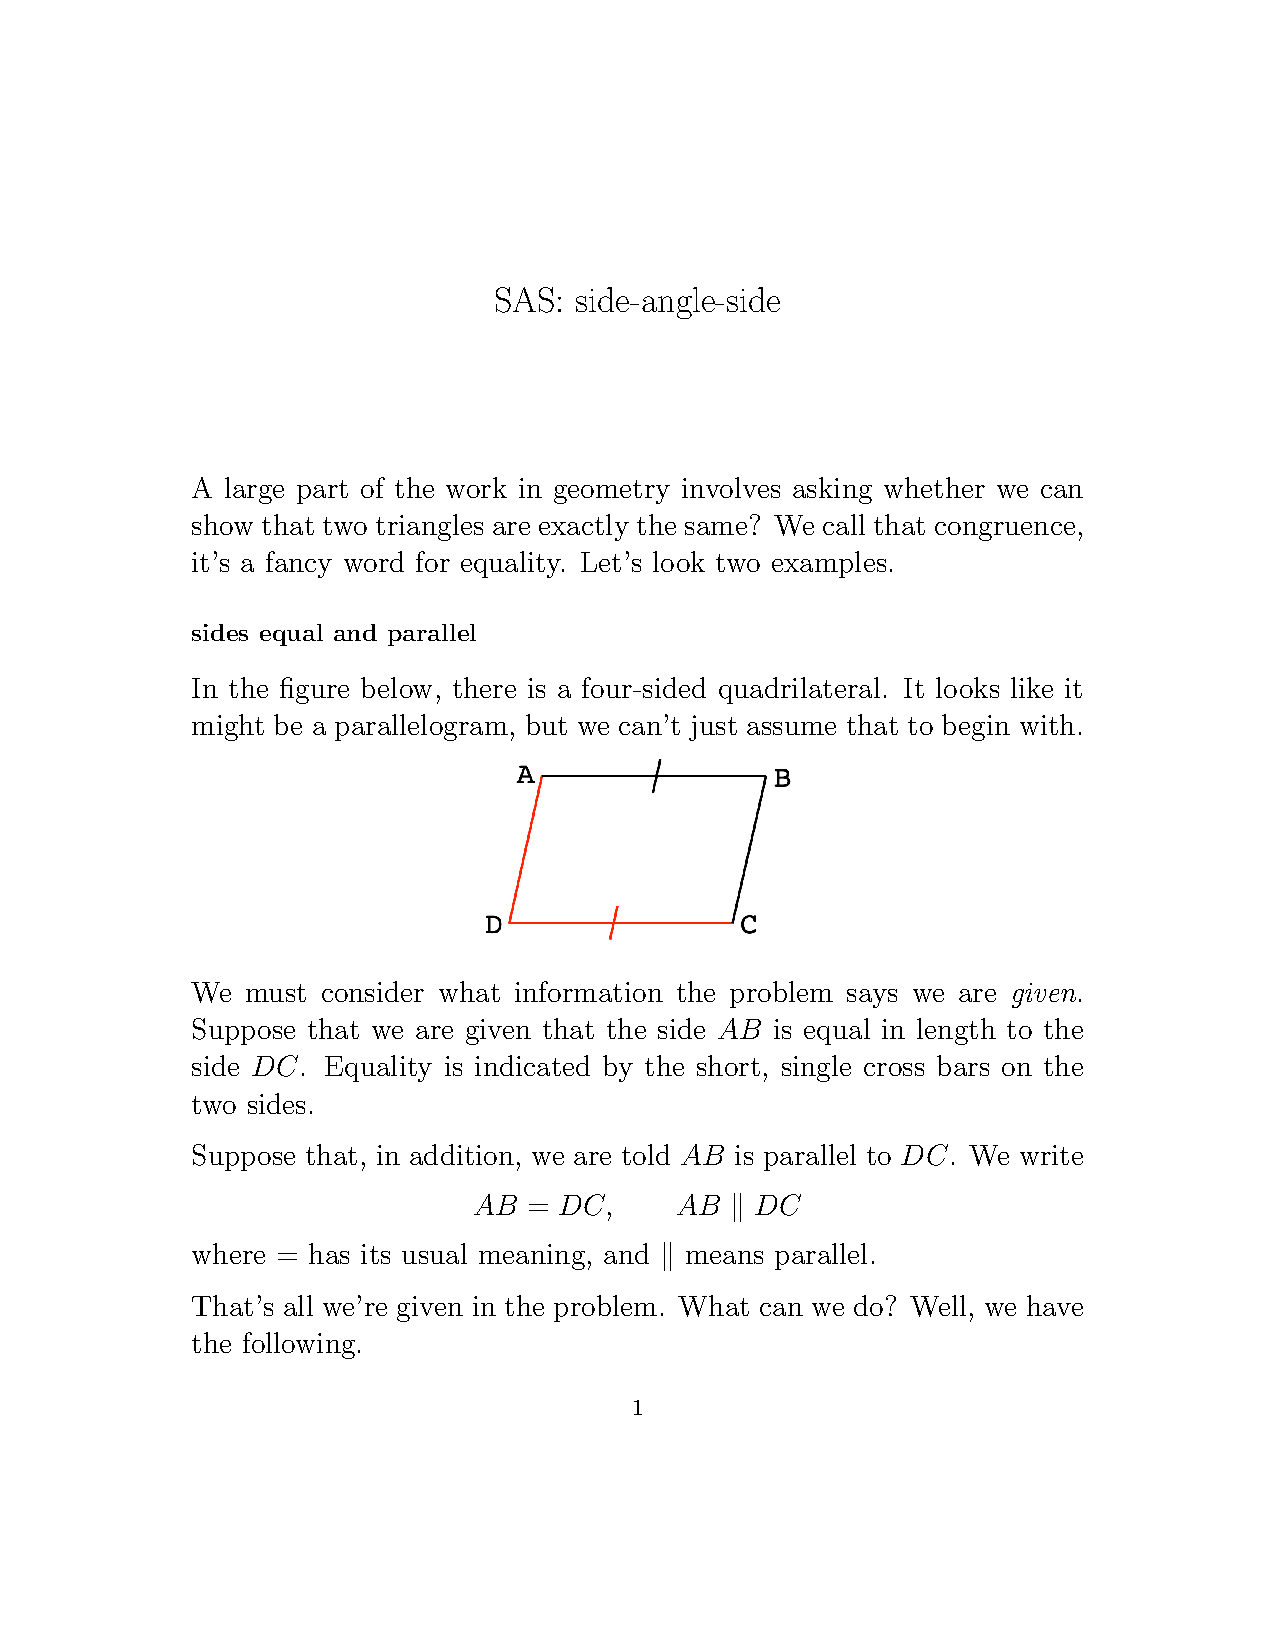
\includegraphics [scale=0.4] {SAS.png} \end{center}

In this diagram, sides of equal length are indicated by one or more hash marks.  

Equal angles are indicated by dots here. Dots are easier to place on the figures, and lend themselves to color-coding;  the common method for pencil and paper is to draw an arc with a hash across it, or just use a filled and open circle.

ASA
\begin{center} \includegraphics [scale=0.4] {ASA3.png} \end{center}

AAS.
\begin{center} \includegraphics [scale=0.4] {AAS.png} \end{center}

There is one set of three that doesn't work in the general case, that is SSA (side-side-angle).  We don't need to worry about why right now.  One way to remember that SSA is problematic is to write the letters in reverse order:  ASS.

\subsection*{proofs}

We have not formally proved that any of these methods are correct.  Even Euclid encounters some difficulty with this point.  He "proves" SAS by a method that is arguably not a real proof.

You can think of them as axioms if you like.  

We will prove that SAS implies SSS, after first proving a basic theorem about isosceles triangles.  This is one of Thales original theorems.

$\bullet$ \ \ If a triangle has two sides equal (isosceles), then the corresponding opposite base angles are equal.

\emph{Proof}.

Suppose we draw an isosceles triangle with $AB = AC$.  We will prove that the angles that are marked with black dots are actually equal, we don't assume that yet for the proof.

\begin{center} \includegraphics [scale=0.5] {isosceles5.png} \end{center}

We simply divide the angle at the top, vertex $A$ in half.  The line which does this is called the angle bisector.  We extend that line to meet the base, forming $AD$.  Because $AD$ is a bisector, the angles at the top marked with an "x" are equal.

We are given that the sides $AB$ and $AC$ are equal, our construction gives equal angles $\angle BAD$ and $\angle DAC$, and the side $AD$ is shared.  We have SAS, so $\triangle ABD \cong \triangle ACD$.

Since the triangles are congruent, the corresponding angles with the black dots are equal.  Also the angles at the base of the bisector are equal, which means that, since $BC$ is a straight line, the two angles at $D$ are both right angles.  AD is the \emph{altitude} of this triangle.

$\square$

And now

$\bullet$ \ \  SAS $\rightarrow$ SSS.

\emph{Proof}.

We first draw $\triangle ABC$, and then place $D$ so that two sets of sides are equal.  So $AC = AD$ and $AD = BC$.  And we have chosen a particular value for the total angle at vertex $C$.

\begin{center} \includegraphics [scale=0.4] {SSS.png} \end{center}

By the the isosceles triangle theorem, the angles marked with black dots are equal, as are the angles marked with red dots.  Therefore $\angle D = \angle C$.  We have SAS, so $\triangle ABC \cong \triangle ABD$.

And then we just note that side $AB$ is shared.  This means that we have SSS.

$\square$

\end{document}